

\tikzset{every picture/.style={line width=0.75pt}} %set default line width to 0.75pt        

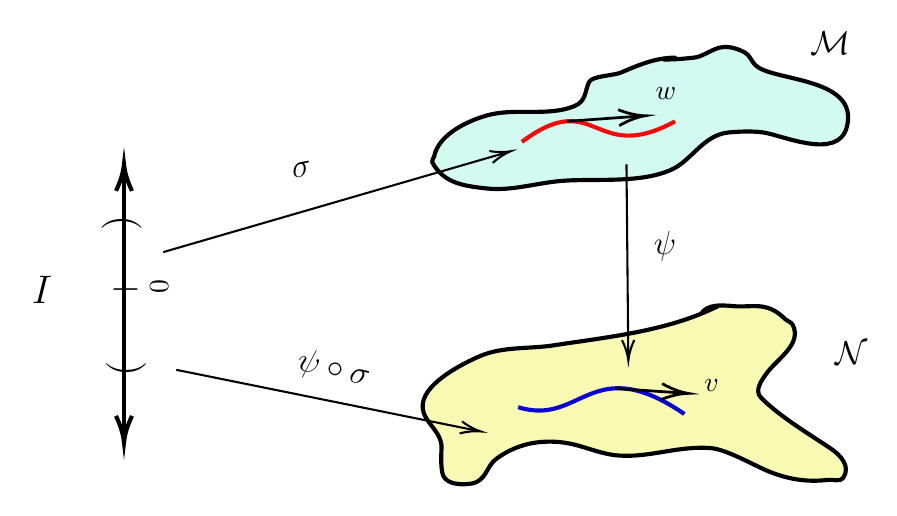
\begin{tikzpicture}[x=0.75pt,y=0.75pt,yscale=-1,xscale=1, scale=0.9]
%uncomment if require: \path (0,300); %set diagram left start at 0, and has height of 300

%Curve Lines [id:da9083608220761967] 
\draw [fill={rgb, 255:red, 130; green, 241; blue, 213 }  ,fill opacity=0.35 ][line width=1.5] [line join = round][line cap = round]   (419,36.9) .. controls (408.53,36.9) and (399.12,40.99) .. (390,44.9) .. controls (386.21,46.52) and (374.64,46.61) .. (373,49.9) .. controls (370.6,54.69) and (371.63,60.25) .. (365,62.9) .. controls (350.57,68.67) and (333.08,63.5) .. (318,67.9) .. controls (307.64,70.92) and (292.38,78) .. (290,89.9) .. controls (289.79,90.93) and (288.5,91.97) .. (289,92.9) .. controls (295.24,104.34) and (306.15,105.58) .. (318,106.9) .. controls (331.56,108.41) and (344.5,104.02) .. (358,102.9) .. controls (375.97,101.4) and (400.01,104.45) .. (417,96.9) .. controls (427.96,92.03) and (434.19,78.05) .. (448,76.9) .. controls (453.98,76.4) and (460.05,76.13) .. (466,76.9) .. controls (476.13,78.21) and (506.38,92.36) .. (511,73.9) .. controls (517.73,46.99) and (470.81,49.71) .. (462,40.9) .. controls (459.58,38.48) and (459.1,35.45) .. (456,33.9) .. controls (441.6,26.7) and (437.76,35.93) .. (429,36.9) .. controls (423.69,37.49) and (418.34,37.9) .. (413,37.9) ;
%Curve Lines [id:da9706399412764172] 
\draw [fill={rgb, 255:red, 243; green, 245; blue, 132 }  ,fill opacity=0.62 ][line width=1.5] [line join = round][line cap = round]   (442,169.9) .. controls (415.05,183.38) and (383.37,186.38) .. (354,190.9) .. controls (340.55,192.97) and (326.73,191.3) .. (314,196.9) .. controls (306.4,200.25) and (285.66,210.3) .. (284,221.9) .. controls (282.65,231.35) and (293.45,235.57) .. (294,244.9) .. controls (294.07,246.04) and (293.14,257.18) .. (295,260.9) .. controls (297.5,265.91) and (306.04,265.51) .. (310,264.9) .. controls (317.87,263.69) and (318.03,255.62) .. (323,251.9) .. controls (333.48,244.04) and (345.73,241.24) .. (359,242.9) .. controls (369.41,244.2) and (378.48,249.2) .. (389,249.9) .. controls (405.91,251.03) and (420.22,244.63) .. (438,245.9) .. controls (446.16,246.48) and (460.54,254.7) .. (468,257.9) .. controls (479.08,262.65) and (489.81,264.3) .. (501,262.9) .. controls (503.67,262.57) and (507.51,264.14) .. (509,261.9) .. controls (513.11,255.74) and (507.94,249.86) .. (502,245.9) .. controls (488.72,237.05) and (474.94,228.84) .. (465,218.9) .. controls (461.14,215.04) and (465.67,209.16) .. (468,205.9) .. controls (473.43,198.29) and (487.24,190.37) .. (482,179.9) .. controls (481.25,178.41) and (479.18,178.08) .. (478,176.9) .. controls (467.95,166.85) and (460.57,170.86) .. (450,169.9) .. controls (443.82,169.34) and (436.45,168.73) .. (433,173.9) ;
%Straight Lines [id:da7589756419214643] 
\draw [line width=1.5]    (124,97) -- (124,239.9) ;
\draw [shift={(124,242.9)}, rotate = 270] [color={rgb, 255:red, 0; green, 0; blue, 0 }  ][line width=1.5]    (14.21,-4.28) .. controls (9.04,-1.82) and (4.3,-0.39) .. (0,0) .. controls (4.3,0.39) and (9.04,1.82) .. (14.21,4.28)   ;
\draw [shift={(124,94)}, rotate = 90] [color={rgb, 255:red, 0; green, 0; blue, 0 }  ][line width=1.5]    (14.21,-4.28) .. controls (9.04,-1.82) and (4.3,-0.39) .. (0,0) .. controls (4.3,0.39) and (9.04,1.82) .. (14.21,4.28)   ;
%Straight Lines [id:da15285926618261458] 
\draw    (145,141) -- (329.08,87.56) ;
\draw [shift={(331,87)}, rotate = 163.81] [color={rgb, 255:red, 0; green, 0; blue, 0 }  ][line width=0.75]    (10.93,-3.29) .. controls (6.95,-1.4) and (3.31,-0.3) .. (0,0) .. controls (3.31,0.3) and (6.95,1.4) .. (10.93,3.29)   ;
%Straight Lines [id:da4966374031544514] 
\draw    (152,204) -- (313.04,236.6) ;
\draw [shift={(315,237)}, rotate = 191.45] [color={rgb, 255:red, 0; green, 0; blue, 0 }  ][line width=0.75]    (10.93,-3.29) .. controls (6.95,-1.4) and (3.31,-0.3) .. (0,0) .. controls (3.31,0.3) and (6.95,1.4) .. (10.93,3.29)   ;
%Curve Lines [id:da714564075847796] 
\draw [color={rgb, 255:red, 245; green, 9; blue, 9 }  ,draw opacity=1 ][line width=1.5]    (337,82) .. controls (377,52) and (375,95) .. (419,71) ;
%Curve Lines [id:da26538820278083086] 
\draw [color={rgb, 255:red, 9; green, 5; blue, 211 }  ,draw opacity=1 ][line width=1.5]    (335,224) .. controls (369,234.62) and (374,193.62) .. (424,227.62) ;
%Straight Lines [id:da20362367095818434] 
\draw    (393,94) -- (393.98,197) ;
\draw [shift={(394,199)}, rotate = 269.45] [color={rgb, 255:red, 0; green, 0; blue, 0 }  ][line width=0.75]    (10.93,-3.29) .. controls (6.95,-1.4) and (3.31,-0.3) .. (0,0) .. controls (3.31,0.3) and (6.95,1.4) .. (10.93,3.29)   ;
%Straight Lines [id:da09726797419252065] 
\draw [line width=1.0]    (361,71) -- (400.01,68.21) ;
\draw [shift={(403,68)}, rotate = 175.91] [color={rgb, 255:red, 0; green, 0; blue, 0 }  ][line width=1.0]    (14.21,-4.28) .. controls (9.04,-1.82) and (4.3,-0.39) .. (0,0) .. controls (4.3,0.39) and (9.04,1.82) .. (14.21,4.28)   ;
%Straight Lines [id:da4554197621882127] 
\draw [line width=1.0]    (387,214) -- (423.01,216.42) ;
\draw [shift={(426,216.62)}, rotate = 183.84] [color={rgb, 255:red, 0; green, 0; blue, 0 }  ][line width=1.0]    (14.21,-4.28) .. controls (9.04,-1.82) and (4.3,-0.39) .. (0,0) .. controls (4.3,0.39) and (9.04,1.82) .. (14.21,4.28)   ;

% Text Node
\draw (135.1,119.5) node [anchor=north west][inner sep=0.75pt]  [font=\Large,rotate=-90]  {$($};
% Text Node
\draw (112.9,209.5) node [anchor=north west][inner sep=0.75pt]  [font=\Large,rotate=-270]  {$($};
% Text Node
\draw (115,152.4) node [anchor=north west][inner sep=0.75pt]  [font=\Large]  {$-$};
% Text Node
\draw (136.4,165) node [anchor=north west][inner sep=0.75pt]  [font=\normalsize,rotate=-270]  {$0$};
% Text Node
\draw (73,152.4) node [anchor=north west][inner sep=0.75pt]  [font=\Large]  {$I$};
% Text Node
\draw (490,21.4) node [anchor=north west][inner sep=0.75pt]  [font=\large]  {$\mathcal{M}$};
% Text Node
\draw (503,187.4) node [anchor=north west][inner sep=0.75pt]  [font=\large]  {$\mathcal{N}$};
% Text Node
\draw (406,128.4) node [anchor=north west][inner sep=0.75pt]  [font=\large]  {$\psi $};
% Text Node
\draw (211.36,92.75) node [anchor=north west][inner sep=0.75pt]  [font=\large,rotate=-349.5]  {$\sigma $};
% Text Node
\draw (217.82,189.56) node [anchor=north west][inner sep=0.75pt]  [font=\large,rotate=-13.4]  {$\psi \circ \sigma $};
% Text Node
\draw (433,207.4) node [anchor=north west][inner sep=0.75pt]    {$v$};
% Text Node
\draw (407,51.4) node [anchor=north west][inner sep=0.75pt]    {$w$};


\end{tikzpicture}
